





\begin{figure}
   \centering
   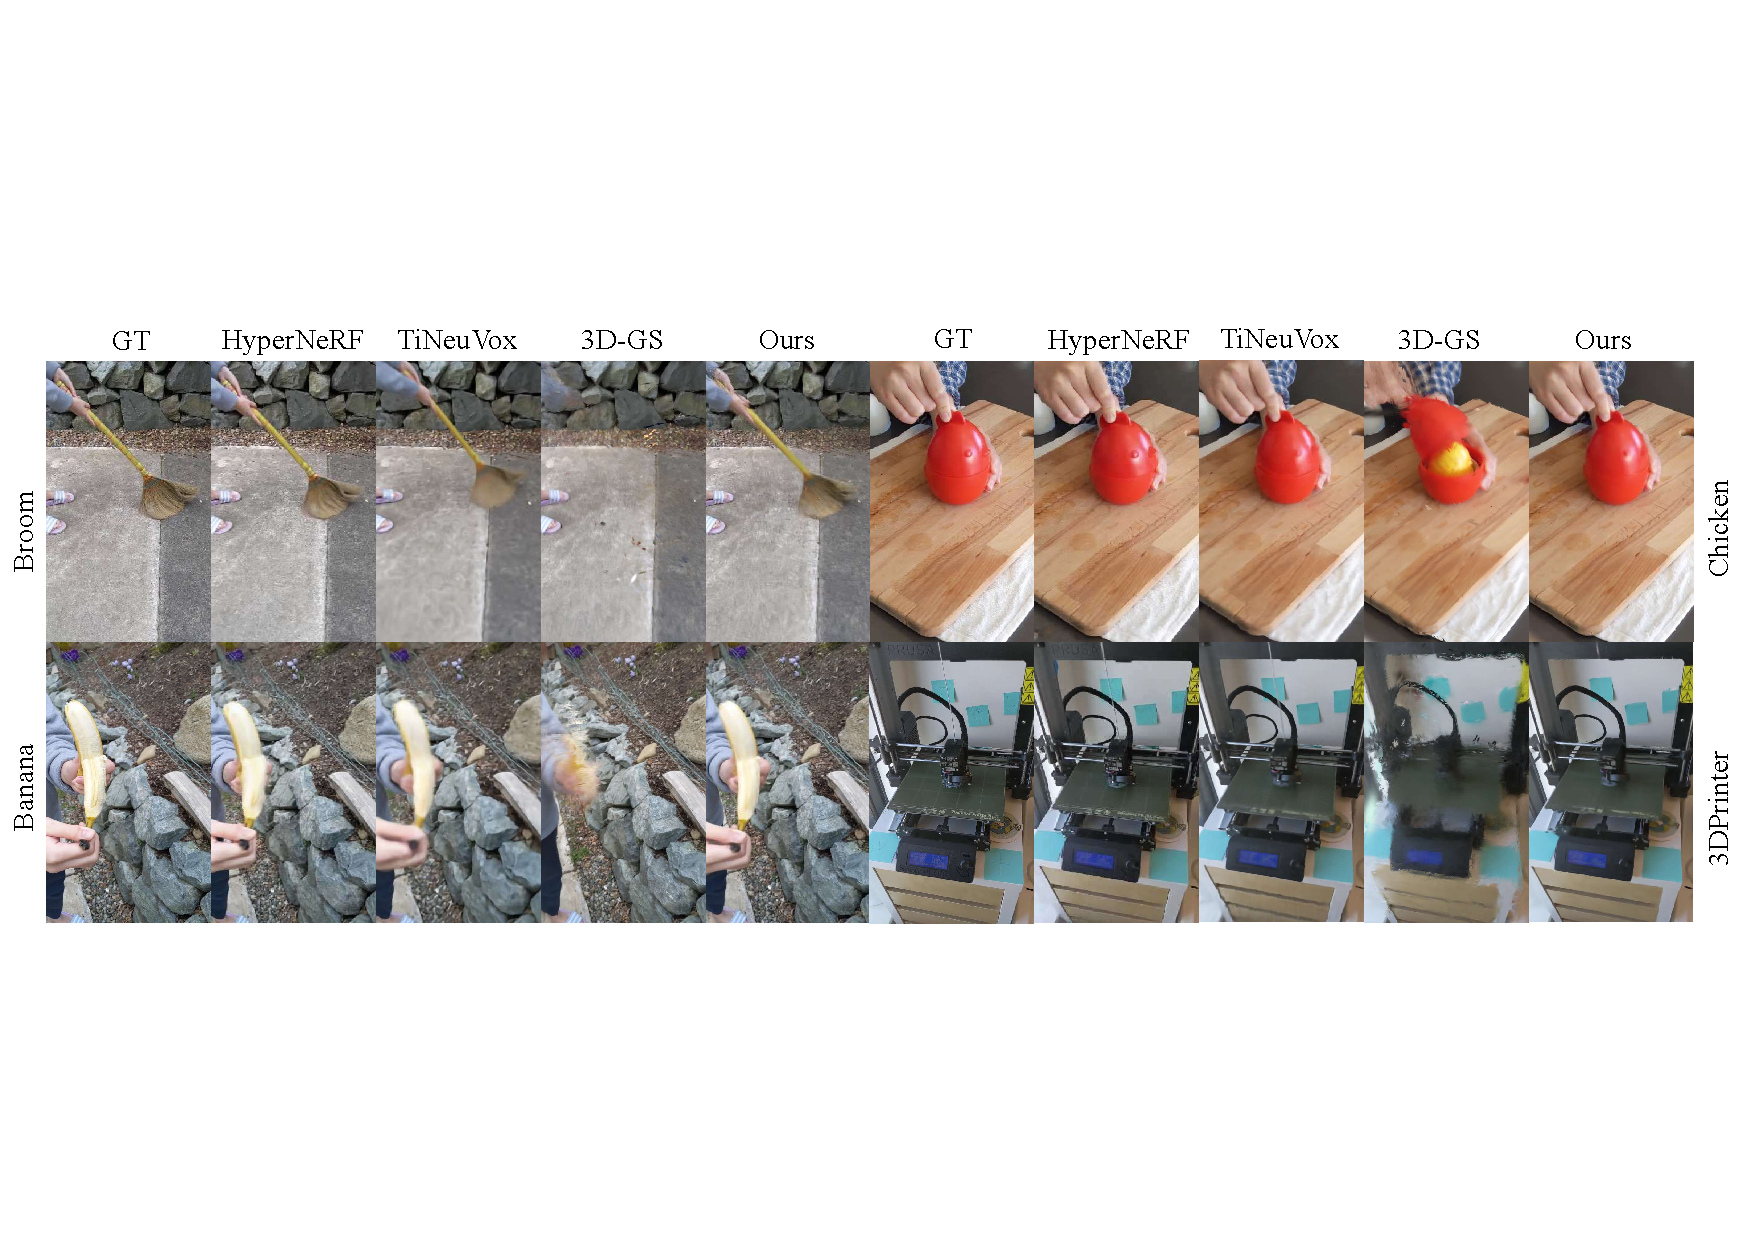
\includegraphics[width=0.95\linewidth]{fig/hyper_result.pdf}
    \caption{Visualization of the HyperNeRF~\cite{park2021hypernerf} datasets compared with other methods~\cite{3dgs,park2021hypernerf,tineuvox,guo2023forwardflowfornvs}. `GT' stands for ground truth images.}
      \label{fig:hyper_result}
    \vspace{-20pt}
\end{figure}


\begin{figure}
   \centering
   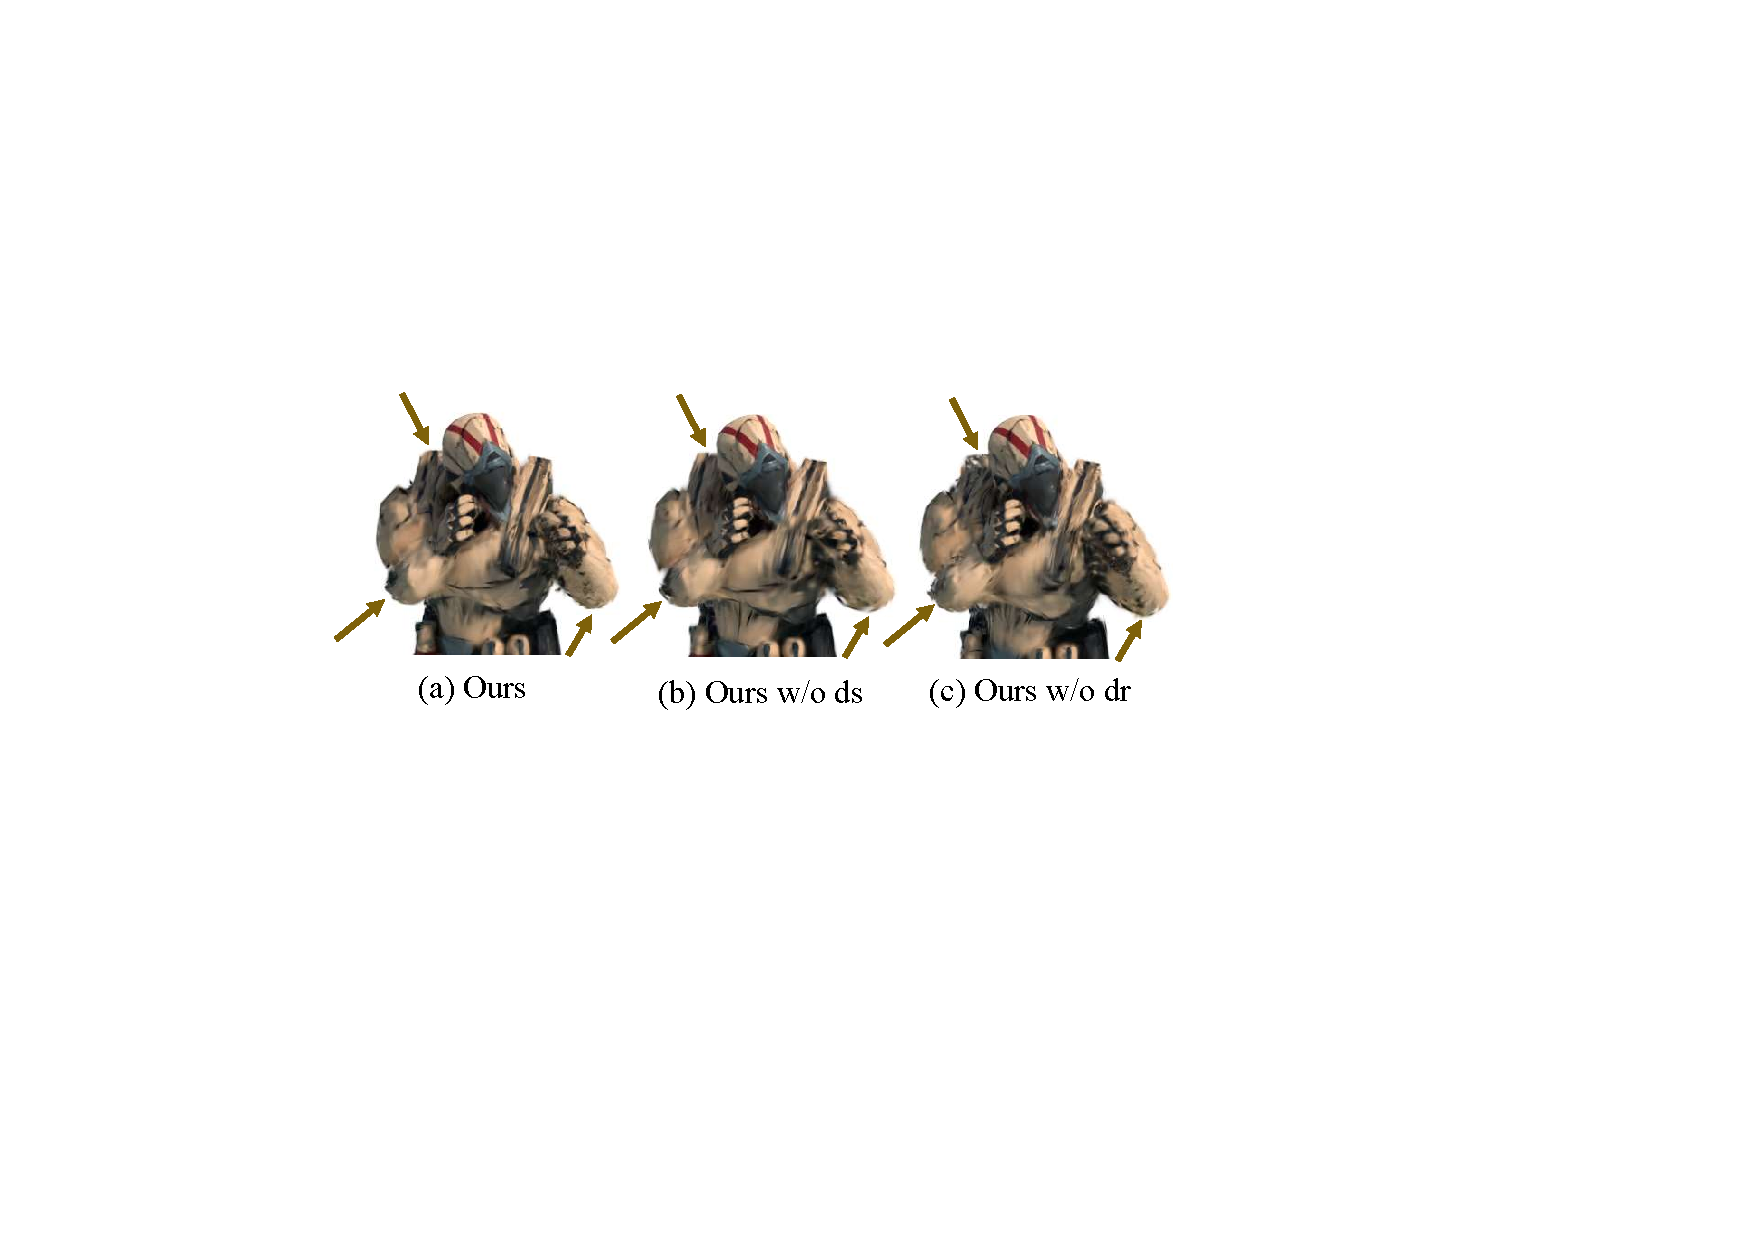
\includegraphics[width=0.9\linewidth]{fig/ab_nodrdx.pdf}
   \caption{Ablation Study of the rotation and scaling decoder. `ds'  denotes as $\phi_s$ and, `'dr' stands for $\phi_r$.}
      \label{fig:ab_nodrdx}
    \vspace{-10pt}
\end{figure}










\begin{table*} 
\small
\centering
\caption{Quantitative results on the synthesis dataset. The \colorbox{pink}{best} and the \colorbox{yellow}{second best} results are denoted by pink and yellow. The rendering resolution is set to 800$\times$800. ``Time'' in the table stands for training times.}
\setlength{\tabcolsep}{10pt}
\begin{tabular}{l|ccc|c|cc} 
\toprule
Model  & PSNR(dB)↑ & SSIM↑ & LPIPS↓ & Time↓ &  FPS ↑ & Storage (MB)↓  \\
\midrule  
TiNeuVox-B~\cite{tineuvox}  & 32.67 & 0.97 &  0.04 & 28 mins & 1.5 & 48\\ 
KPlanes~\cite{kplanes} & 31.61 & 0.97 &-& 52 mins& 0.97   &418\\ 
HexPlane-Slim~\cite{hexplane} & 31.04 & 0.97 & 0.04&11m 30s& 2.5 &38\\ 
3D-GS~\cite{3dgs} &23.19 & 0.93 & 0.08&10 mins  \cellcolor{yellow}&\cellcolor{pink}170&\cellcolor{pink}10 \\

FFDNeRF~\cite{guo2023forwardflowfornvs}&\cellcolor{yellow}32.68&0.97&0.04&-&$<$ 1&440\\

MSTH~\cite{msth}&31.34&\cellcolor{yellow}0.98&\cellcolor{yellow}0.02&\cellcolor{pink}6 mins&-&-\\
Ours & \cellcolor{pink}34.05&\cellcolor{pink}0.98 &\cellcolor{pink}0.02\cellcolor{pink}& 20 mins&\cellcolor{yellow}82 &\cellcolor{yellow}18 \\
\bottomrule
\end{tabular}  

\label{table_dnerf}
\end{table*}

\begin{table*} 
\centering
\small
\caption{Quantitative results on HyperNeRF's~\cite{park2021hypernerf} vrig dataset. Rendering resolution is set to 960$\times$540.}
\setlength{\tabcolsep}{13pt}
\begin{tabular}{l|cc|c|cc} 
\toprule  
Model  & PSNR(dB)↑ & MS-SSIM↑  & Times↓ &  FPS↑ & Storage(MB)↓\\ 
\midrule  
Nerfies~\cite{park2021nerfies}&22.2&0.803&$\sim$ hours&$<$ 1&-\\
HyperNeRF~\cite{park2021hypernerf}&22.4&0.814&32 hours &$<$ 1&-\\
TiNeuVox-B~\cite{tineuvox}&\cellcolor{yellow}24.3&0.836&\cellcolor{pink}30 mins&1&\cellcolor{pink}48\\
3D-GS~\cite{3dgs}&19.7&0.680&\cellcolor{yellow}40 mins&\cellcolor{pink}55&\cellcolor{yellow}52\\
FFDNeRF~\cite{guo2023forwardflowfornvs}&24.2&\cellcolor{yellow}0.842&-&0.05&440\\
Ours&\cellcolor{pink}25.2&\cellcolor{pink}0.845&1 hour& \cellcolor{yellow}34&61\\
\bottomrule
\end{tabular}  
\label{tab:hypernerf}
\end{table*}


\begin{table*} 
\centering
\caption{Quantitative results on the Neu3D's~\cite{li2022neural} dataset, rendering resolution is set to 1352$\times$1014.}
\setlength{\tabcolsep}{8pt}
\begin{tabular}{l|ccc|c|cc}  
\toprule
Model  & PSNR(dB)↑ & D-SSIM↓ & LPIPS↓ & Time ↓  & FPS↑ & Storage (MB)↓ \\ 
\midrule 
% Neural Volumes  & 22.800 & 0.062 & 0.295 & - & 1352 × 1014 &- &- \\ 
% LLFF & 23.239 & 0.076 & 0.235 & -& 1352 × 1014&-\\ 
% NeRF-T  & 28.449 & 0.023 & 0.100 &- &1352 × 1014 & 0.011&-\\ 
% DyNeRF  & 29.581 & 0.020 & 0.099 & 1344 hours &1352 × 1014&0.011&- \\  
NeRFPlayer~\cite{song2023nerfplayer}  & 30.69 &  0.034  & 0.111  &  6 hours& 0.045&-\\  
HyperReel~\cite{attal2023hyperreel} &31.10&0.036&0.096&9 hours&2.0&360\\
% K-Planes&31.63&0.018&-&108 mins&-&-&
% HexPlane   & 29.470 & 0.018 & 0.078 & 12 hours &1024 × 768&- &-\\ 
% Ours-batch1*& \textbf{31.15} & 0.9388 &0.1375 & 40 mins  & 30 & 150 M\\
% MixVoxels-L1& 30.80 &0.960&  -  &    1.3 hours&  -&-&-&\\
HexPlane-all*~\cite{hexplane} & 31.70 & \cellcolor{pink}0.014 & 0.075 & 12 hours &0.2&250\\ 
KPlanes~\cite{kplanes}& 31.63& -   &  - &   1.8 hours  &0.3&309\\
Im4D~\cite{lin2023im4d}&\cellcolor{pink}32.58&-&0.208&\cellcolor{yellow}28 mins&$\sim$5&\cellcolor{yellow}93\\
MSTH~\cite{msth}&\cellcolor{yellow}32.37&\cellcolor{yellow}0.015&\cellcolor{yellow}0.056&\cellcolor{pink}20 mins & \cellcolor{yellow}2(15$^\ddag$)&135\\
Ours& 31.15 & 0.016 &\cellcolor{pink}0.049 & 40 mins  &\cellcolor{pink}30 & \cellcolor{pink}90\\
\hline  
\end{tabular}  

 \begin{tablenotes}
        \footnotesize
        \item[*] *: The metrics of the model are tested without ``coffee martini'' and resolution is set to 1024$\times$768. 
        \item [$^\ddag$] $^\ddag$: The FPS is tested with fixed-view rendering.
        \end{tablenotes}\label{tab:dynerf}

\end{table*}

\begin{table*} 
\centering


\caption{Ablation studies on synthetic datasets using our proposed methods.}

% \resizebox{\linewidth}{!}{
% \setlength{\tabcolsep}{0pt} % 缩小列之间的间距

\begin{tabular}{l|ccc|c|ccc} 
\toprule
Model  & PSNR(dB)↑ & SSIM↑ & LPIPS↓ & Time↓ &FPS↑& Storage (MB)↓&\\
\midrule 
Ours w/o HexPlane $R_l(i,j)$ & 27.05 & 0.95 & 0.05& \cellcolor{pink}10 mins &\cellcolor{pink}140 &\cellcolor{pink}12 \\ 
Ours w/o initialization  &31.91 & 0.97 & 0.03&\cellcolor{yellow}19 mins& 79&18 \\ 
Ours w/o $\phi_x$ &26.67&0.95&0.07&20 mins&82&17\\
Ours w/o $\phi_r$ &33.08\cellcolor{yellow}&\cellcolor{yellow}0.98&\cellcolor{yellow}0.03&20 mins&83\cellcolor{yellow}&\cellcolor{yellow}17\\
Ours w/o $\phi_s$ &33.02&0.98&0.03&20 mins&82&17\\ 
Ours & \cellcolor{pink}34.05&\cellcolor{pink}0.98 &\cellcolor{pink}0.02&20 mins&82 &18 \\

\bottomrule
\end{tabular}  
% }
\label{table_ab}
\vspace{-10pt}
\end{table*}


\section{Experiment}

In this section, we mainly introduce the hyperparameters and datasets of our settings in Sec.~\ref{Experimental Setting} and the results between different datasets will be compared with \cite{tineuvox,msth,wang2023mixedvoxels,lin2023im4d,attal2023hyperreel,hexplane,kplanes,3dgs,song2023nerfplayer} in Sec.~\ref{subsec:result}. Then, ablation studies are proposed to prove the effectiveness of our approaches in Sec.~\ref{subsec:ablation study} and more discussion about 4D-GS in Sec.~\ref{subsec:discussions}. Finally, we discuss the limitation of our proposed 4D-GS in Sec.~\ref{Subsec:limitation}.
\subsection{Experimental Settings}
\label{Experimental Setting}
Our implementation is primarily based on the PyTorch~\cite{pytorch} framework and tested in a single RTX 3090 GPU, and we've fine-tuned our optimization parameters by the configuration outlined in the 3D-GS~\cite{3dgs}. More hyperparameters will be shown in the appendix.
% Notably, we have configured the intervals for point cloud pruning to be set at 8000, and the total training iterations decrease to 20000. Additionally, we have established the voxel plane resolution as $[64,64]$, integrating multi-resolution upsampling at levels  $L = \{2,4,8\}$. Following a similar approach to that elucidated in ~\cite{fridovich2023k}, each plane is endowed with hidden features set to a dimension of 32.

% Moreover, the default setting for the hidden layer of the MLP decoder is 64, and the learning rate is initially set at 1.6e-4, gradually decreasing exponentially to 1.6e-6 by the end of the training process. The learning rate for the voxel grid is initialized at 1.6e-3 and exponentially decays to 1.6e-5.

\paragraph{Synthetic Dataset.}We primarily assess the performance of our model using synthetic datasets, as introduced by D-NeRF~\cite{pumarola2021dnerf}. These datasets are designed for monocular settings, although it's worth noting that the camera poses for each timestamp are close to randomly generated. Each scene within these datasets contains dynamic frames, ranging from 50 to 200 in number.
\paragraph{Real-world Datasets.} We utilize datasets provided by HyperNeRF~\cite{park2021hypernerf} and Neu3D's~\cite{li2022neural} as benchmark datasets to evaluate the performance of our model in real-world scenarios. The Nerfies dataset is captured using one or two cameras, following straightforward camera motion, while the Neu3D's dataset is captured using 15 to 20 static cameras, involving extended periods and intricate camera motions. We use the points computed by SfM~\cite{schonberger2016structure} from the first frame of each video in Neu3D's dataset and 200 frames randomly selected in HyperNeRF's.
% \subsection{Metrics}
% \begin{figure}
%    \centering
%    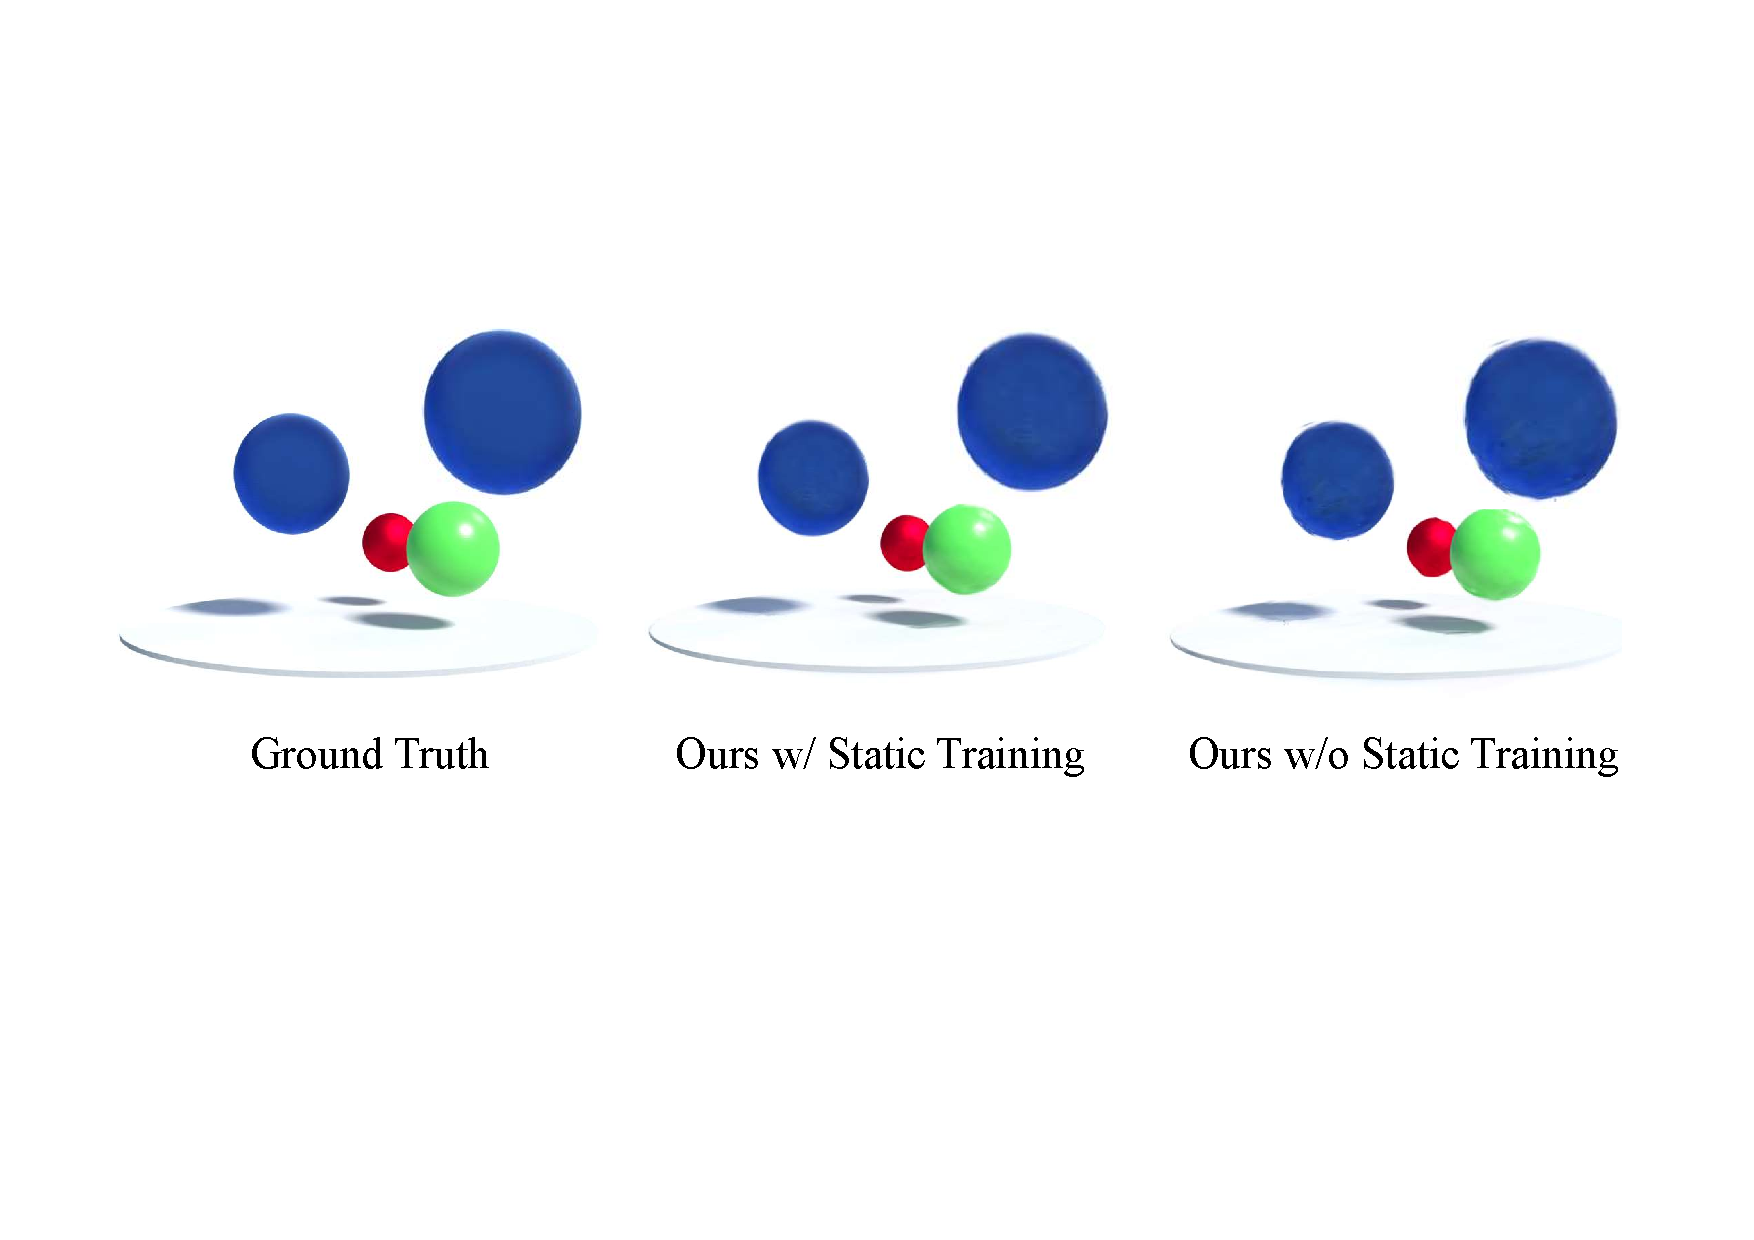
\includegraphics[width=1.0\linewidth]{fig/ab_coarse2fine.pdf}
%    \caption{Ablation Study of two stages training. Without static point cloud initialization, Gaussians may go into local minimum and suffer from a worse quality.}
%    \label{fig: ab_coarse2fine}
% \end{figure}
% \begin{figure}
%    \centering
%    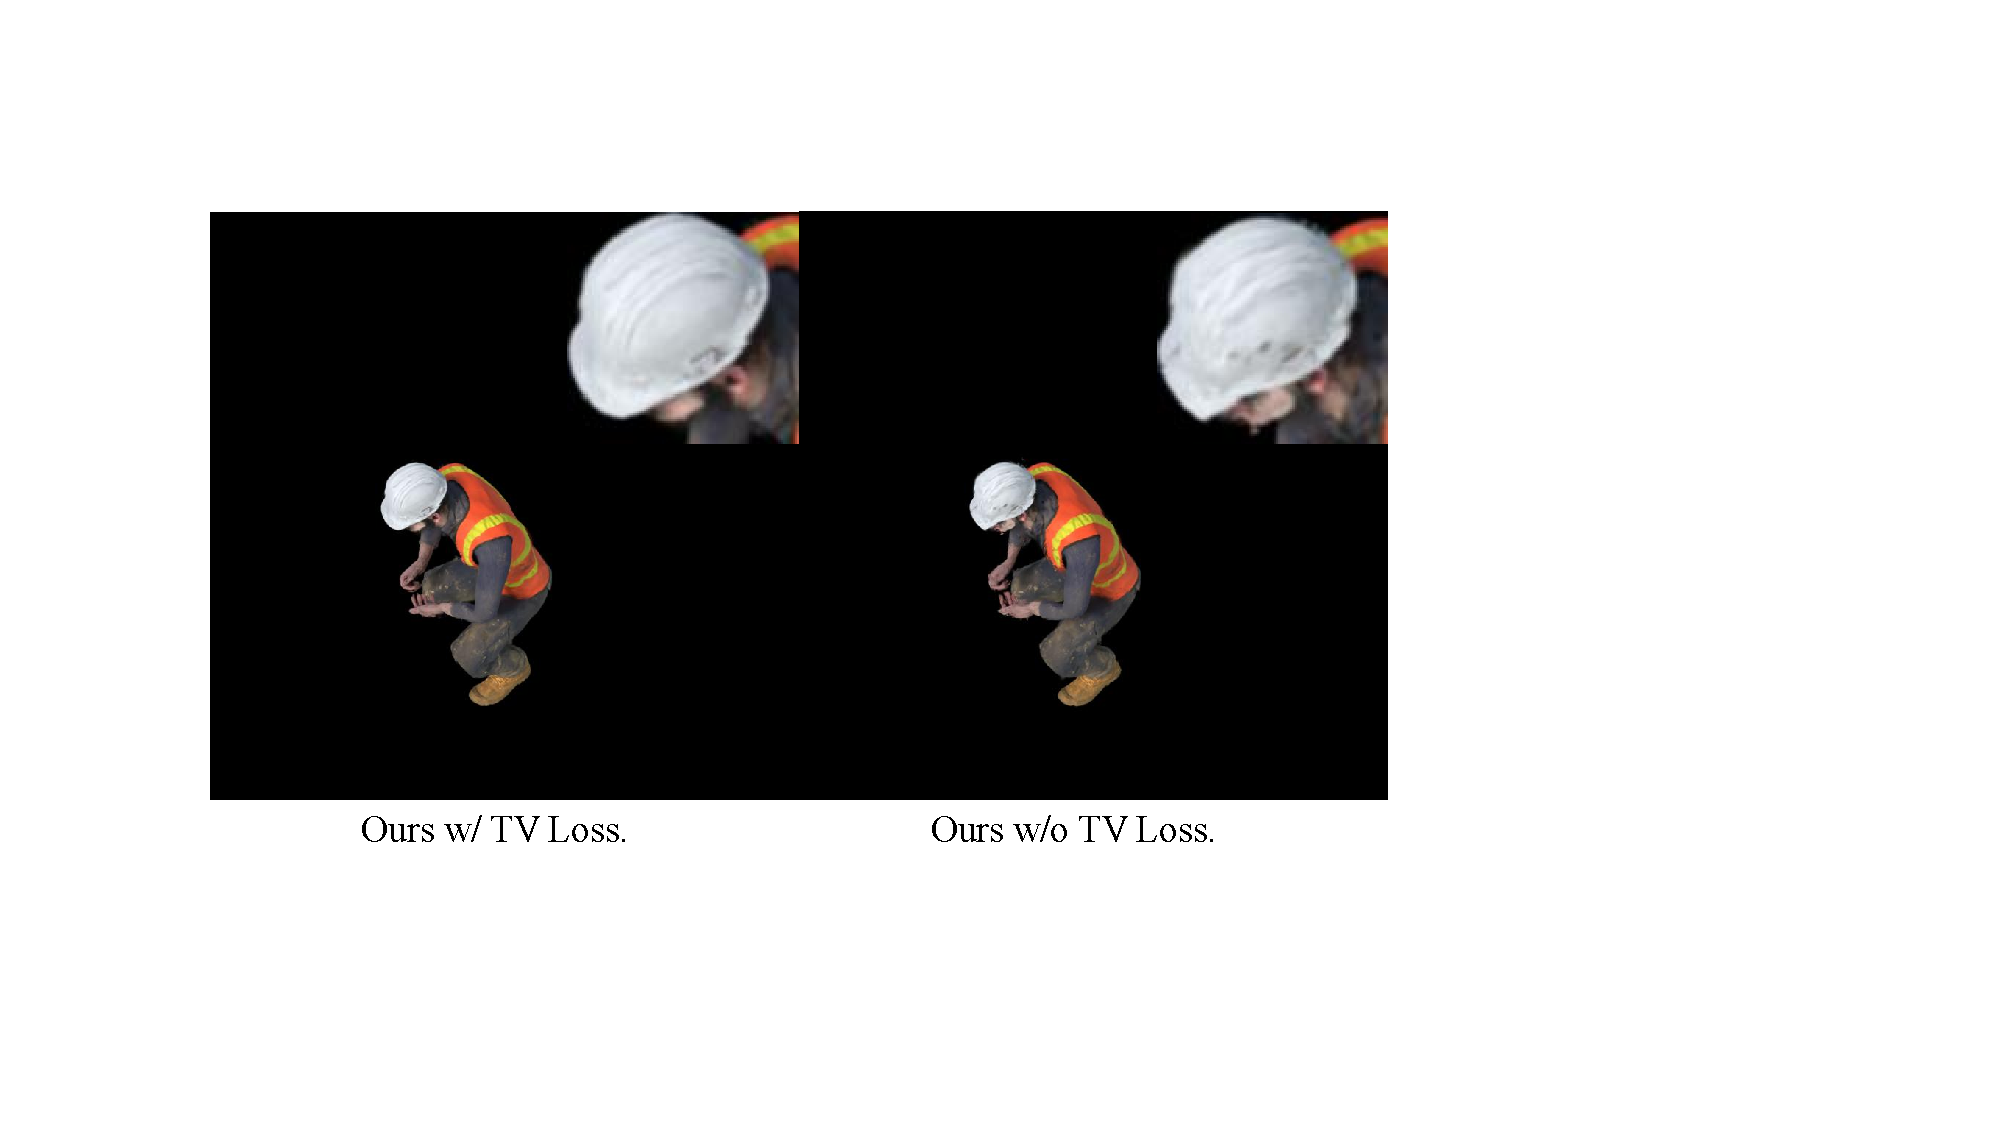
\includegraphics[width=1.0\linewidth]{fig/ab_tv.pdf}
%    \caption{Ablation Study of total variation loss mentioned in ~\cite{kplanes}, with TV loss adopted in voxel grid, the training process will become smoother and enjoy better results.}
%    \label{fig: ab_tv}
% \end{figure}
\subsection{Results}
\label{subsec:result}
We primarily assess our experimental results using various metrics, encompassing peak-signal-to-noise ratio (PSNR), perceptual quality measure LPIPS~\cite{lpips}, structural similarity index (SSIM)~\cite{ssim} and its extensions including structural dissimilarity index measure (DSSIM), multiscale structural similarity index (MS-SSIM), FPS, training times and Storage. 
% Notably, our approach stands out with its relatively swift training pace and exceptionally rapid rendering speed and can handle both monocular and multi-cams setups, achieving over 80 FPS at a resolution of 800$\times$800.

To assess the quality of novel view synthesis, we conducted benchmarking against several state-of-the-art methods in the field, including ~\cite{tineuvox,hexplane,kplanes,msth,3dgs}. The results are summarized in Tab.~\ref{table_dnerf}. While current dynamic hybrid representations can produce high-quality results, they often come with the drawback of rendering speed. The lack of modeling dynamic motion part makes~\cite{3dgs} fail to reconstruct dynamic scenes. In contrast, our method enjoys both the highest rendering quality within the synthesis dataset and exceptionally fast rendering speeds while keeping extremely low storage consumption and convergence time.

Additionally, the results obtained from real-world datasets are presented in Tab.~\ref{tab:hypernerf} and Tab.~\ref{tab:dynerf}. It becomes apparent that some NeRFs~\cite{song2023nerfplayer,attal2023hyperreel,hexplane} suffer from slow convergence speed, and the other grid-based NeRF methods~\cite{tineuvox,hexplane,msth,kplanes} encounter difficulties when attempting to capture intricate object details. In stark contrast, our methods research comparable rendering quality, fast convergence, and excel in free-view rendering speed in indoor cases. Though~\cite{lin2023im4d} addresses the high quality in comparison to ours, the need for multi-cam setups makes it hard to model monocular scenes and other methods also limit free-view rendering speed and storage.
\begin{figure}
   \centering
   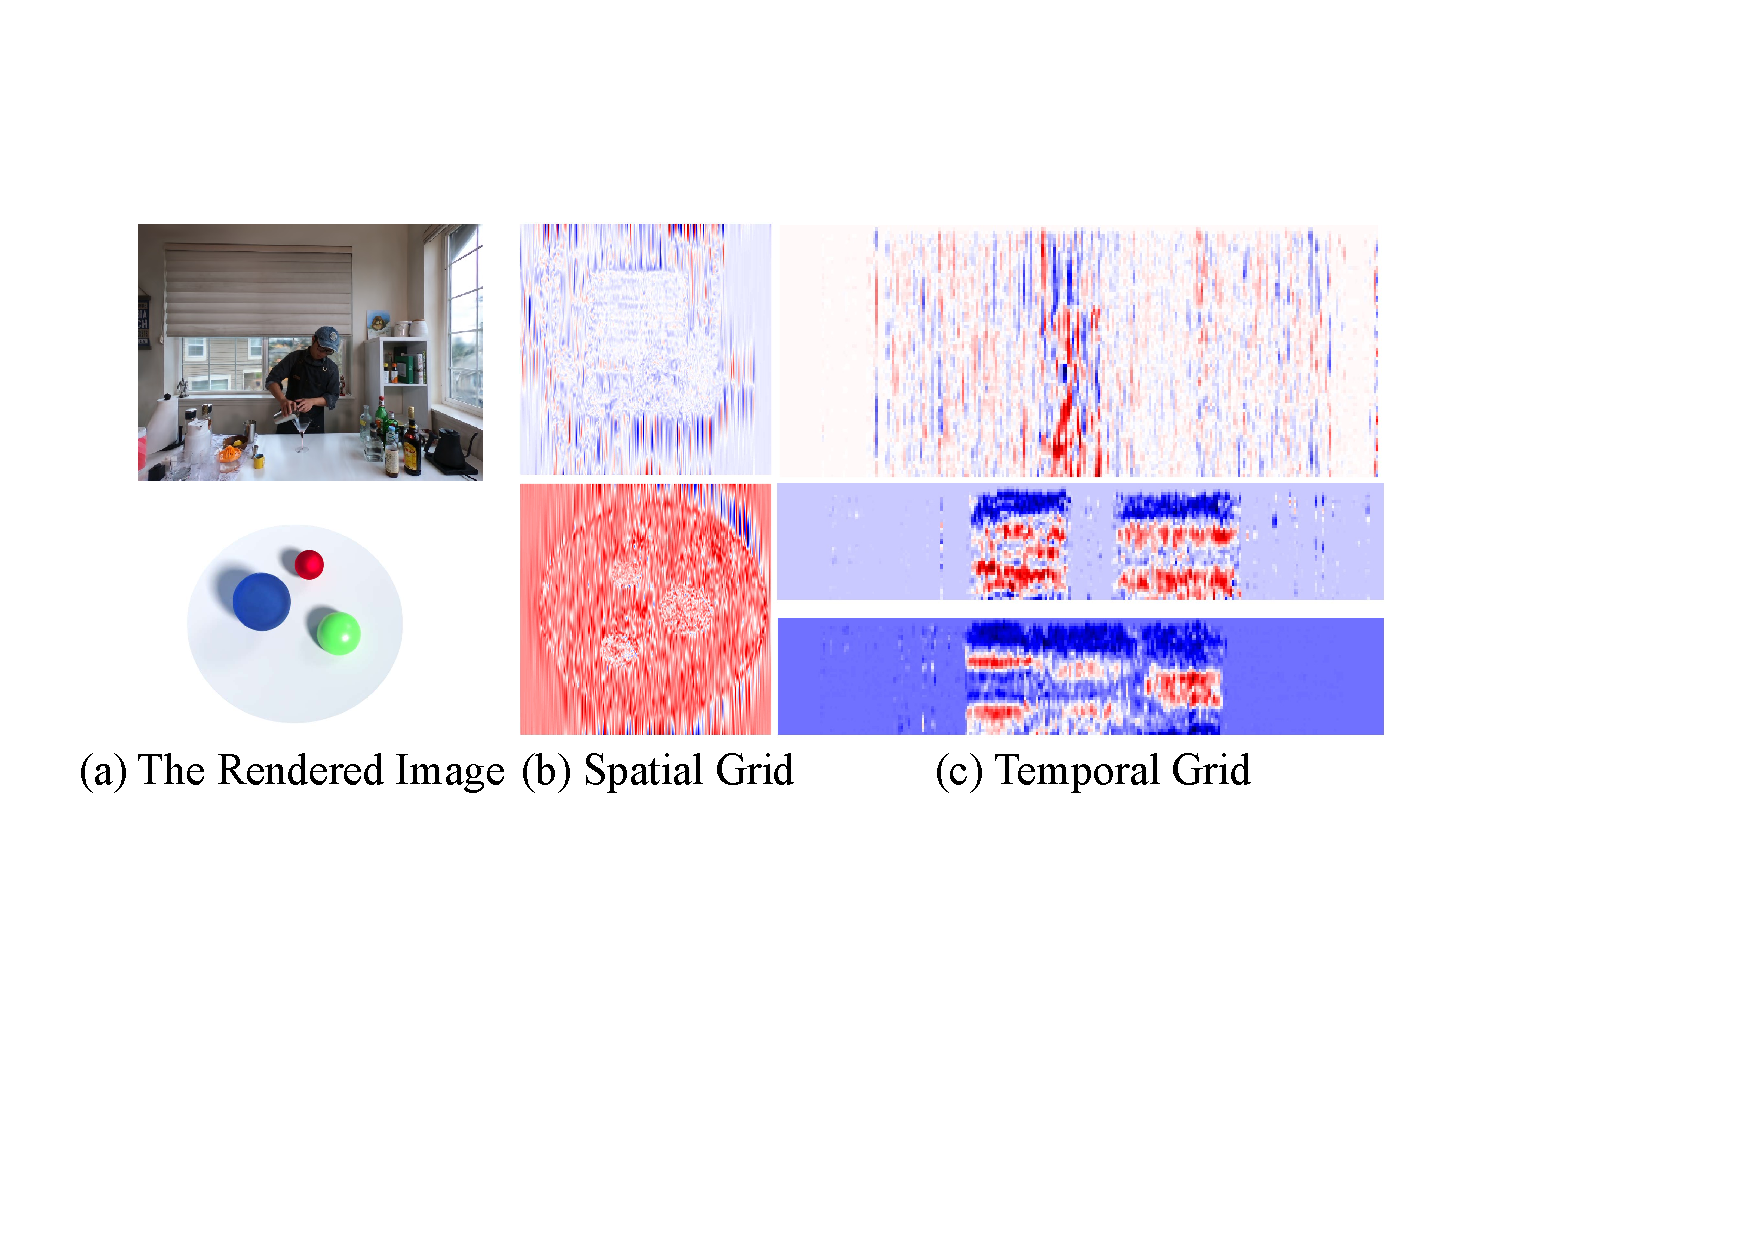
\includegraphics[width=\linewidth]{fig/grid_vis.pdf}
   \caption{Visualization of HexPlane voxel grids. (a) are the rendered images. (b) are the parameters of spatial voxel grids, which implies the feature of 3D Gaussians are encoded in explicit grids. (c) are the temporal features of the grids, each column stands for spatial features in the timestamps.}
   \label{fig: vis_voxelgrid}
\end{figure}

\subsection{Ablation Study}
\label{subsec:ablation study}
\paragraph{Spatial-Temporal Structure Encoder.}
The explicit HexPlane encoder $R_l(i,j)$ possesses the capacity to retain 3D Gaussians' spatial and temporal information, which can reduce storage consumption in comparison with purely explicit methods~\cite{dynamic3dgs}. Discarding this module, we observe that using only a shallow MLP $\phi_d$ falls short in modeling complex deformations across various settings. Tab.~\ref{table_ab} demonstrates that, while the model incurs minimal memory costs, it does come at the expense of rendering quality. 
% \paragraph{Model Capacity.}

% Undoubtedly, expanding the model's size, be it through increased voxel plane resolutions or deeper MLP decoders, can significantly elevate rendering quality. However, this enhancement invariably carries the trade-off of diminished rendering speed, owing to the heightened computational demands imposed by larger models. Tab.~\ref{table_ab} provides concrete evidence of this trade-off. When we augment the hidden layer of the MLP to a size of 256, we observe a noteworthy improvement in rendering quality, translating to an approximate gain of 0.25 dB. 

\vspace{-3pt}
\paragraph{Gaussian Deformation Decoder.}
Our proposed Gaussian deformation decoder $\mathcal{D}$ decodes the features from the spatial-temporal structure encoder $\mathcal{H}$. All the changes in 3D Gaussians can be explained by separate MLPs $\{\phi_x,\phi_r,\phi_s\}$. As is shown in Tab.~\ref{table_ab}, 4D Gaussians cannot fit dynamic scenes well without modeling 3D Gaussian motion. Meanwhile, the movement of human body joints is typically manifested as stretching and twisting of surface details in a macroscopic view. If one aims to accurately model these movements, the size and shape of 3D Gaussians should also be adjusted accordingly. Otherwise, there may be underfitting of details during excessive stretching, or an inability to correctly simulate the movement of objects at a microscopic level.  Fig.~\ref{fig:ab_nodrdx} also demonstrates that shape deformation of 3D Gaussians is important in recovering details.
\vspace{-3pt}
\paragraph{3D Gaussian Initialization.}
In some cases without SfM~\cite{schonberger2016structure} points initialization, training 4D-GS directly may cause difficulty in convergence. Optimizing 3D Gaussians for warm-up enjoys: (a) making some 3D Gaussians stay in the dynamic part, which releases the pressure of large deformation learning by 4D Gaussians as shown in Fig.~\ref{fig: coarse2fine}. (b) learning proper 3D Gaussians $\mathcal{G}$ and suggesting deformation fields paying more attention to the dynamic part like Fig.~\ref{fig: vis_voxelgrid}\textcolor{red} {(c)}. 
(c) avoiding numeric errors in optimizing the Gaussian deformation network $\mathcal{F}$ and keeping the training process stable. Tab.~\ref{table_ab} also shows that if we train our model without the warm-up coarse stage, the rendering quality will suffer.
\subsection{Discussions}\label{subsec:discussions}
\vspace{-3pt}
\paragraph{Analysis of Multi-resolution HexPlane Gaussian Encoder.}The visualization of features in our multi-resolution HexPlane $R_l(i,j)$ is depicted in Fig.~\ref{fig: vis_voxelgrid}. As an explicit module, all the 3D Gaussians features can be easily optimized in individual voxel planes. It can be observed in Fig.~\ref{fig: vis_voxelgrid} \textcolor{red}{(b)} that the voxel plane even shows a similar shape to the rendered image, such as edges. Meanwhile, the temporal features also stay in motion areas in the Fig.~\ref{fig: vis_voxelgrid} \textcolor{red}{(c)}. Such an explicit representation boosts the speed of training and rendering quality of our 4D Gaussians.


\vspace{-3pt}
\begin{figure}
   \centering
   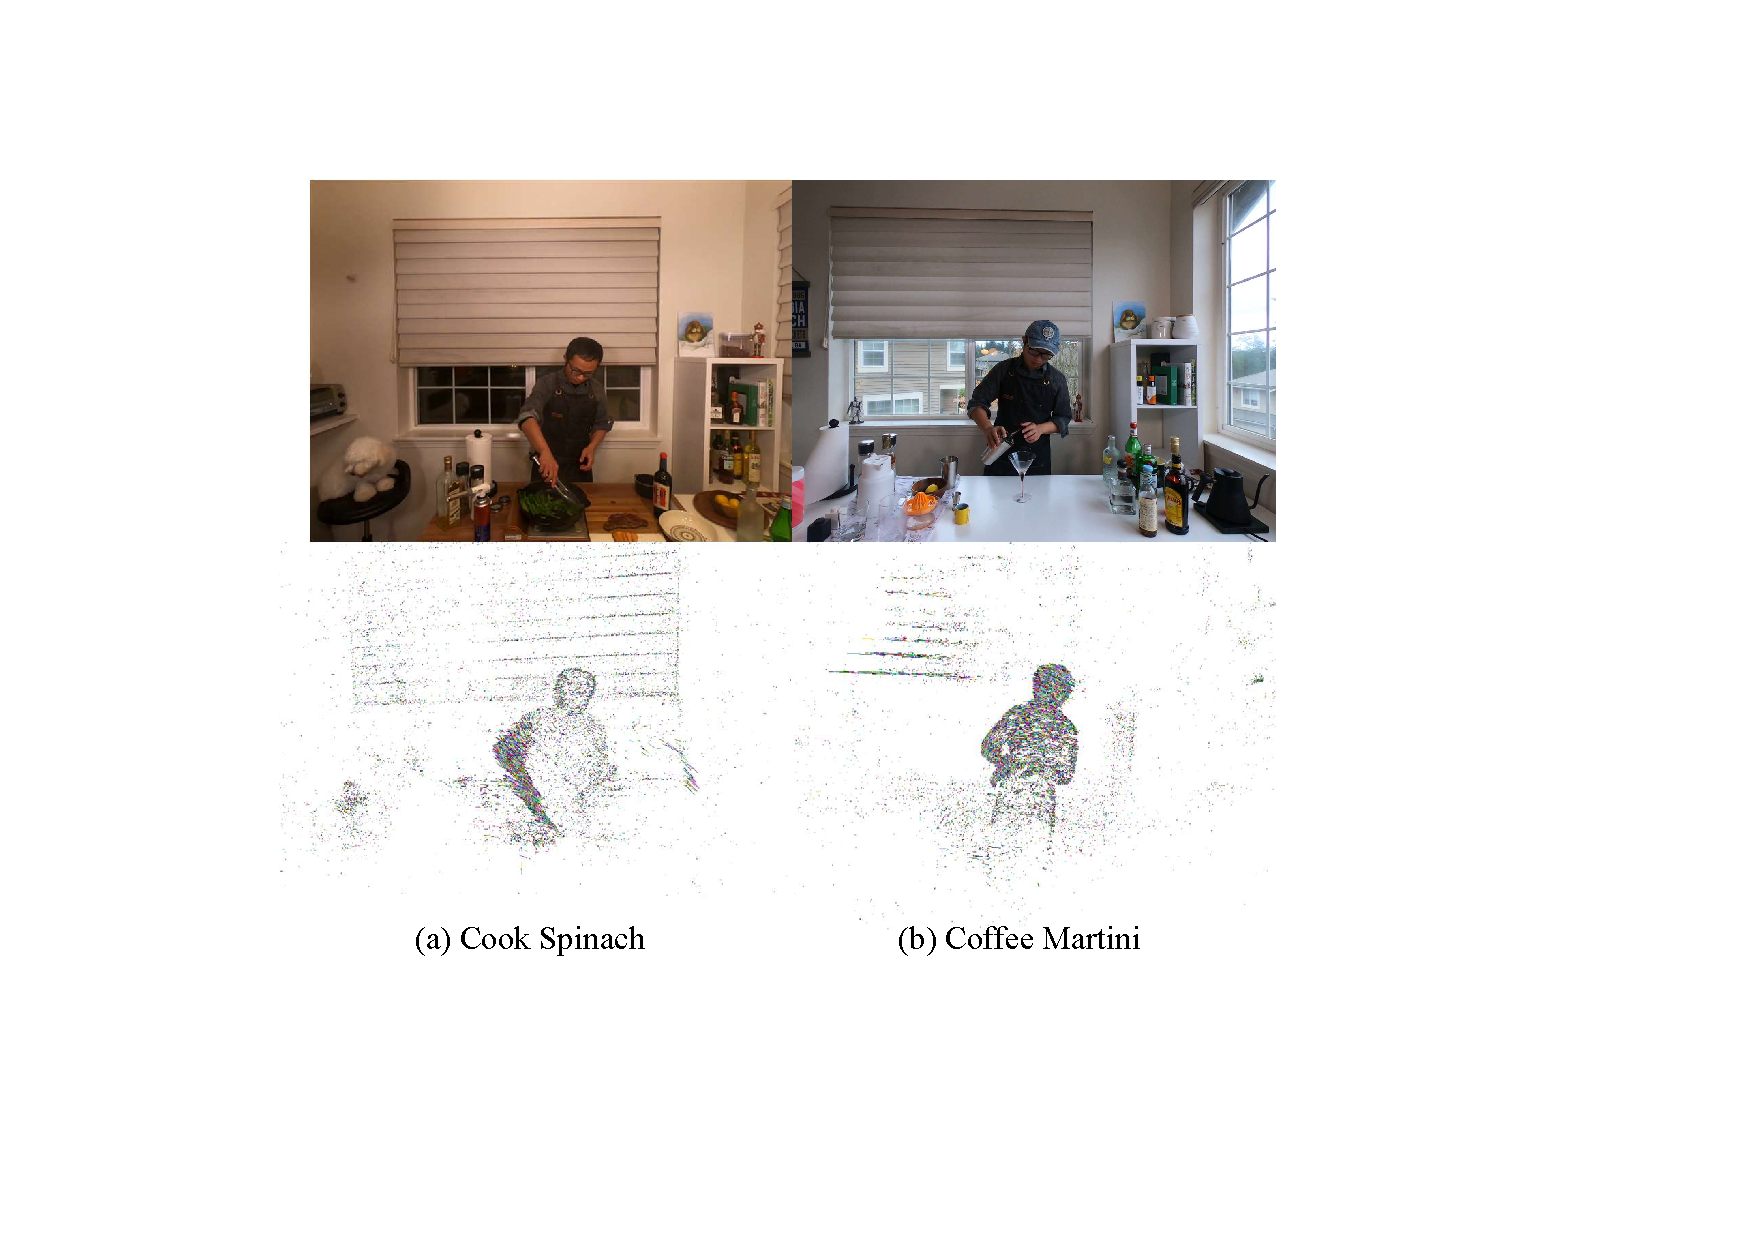
\includegraphics[width=0.9\linewidth]{fig/track_point.pdf}
   \caption{Visualization of tracking with 3D Gaussians. Each line in the figure of second rows stands for trajectories of 3D Gaussians}
      \label{fig:point_track}
\end{figure}

\paragraph{Tracking with 3D Gaussians.}Tracking in 3D is also a important task.~\cite{guo2023forwardflowfornvs} also shows tracking objects' motion in 3D. Different from dynamic3DGS~\cite{dynamic3dgs}, our methods even can present tracking objects in monocular settings with pretty low storage \ie 10MB in 3D Gaussians $\mathcal{G}$ and 8 MB in Gaussian deformation field network $\mathcal{F}$. Fig.~\ref{fig:point_track} shows the 3D Gaussian's deformation at certain timestamps.

\begin{figure}
   \centering
   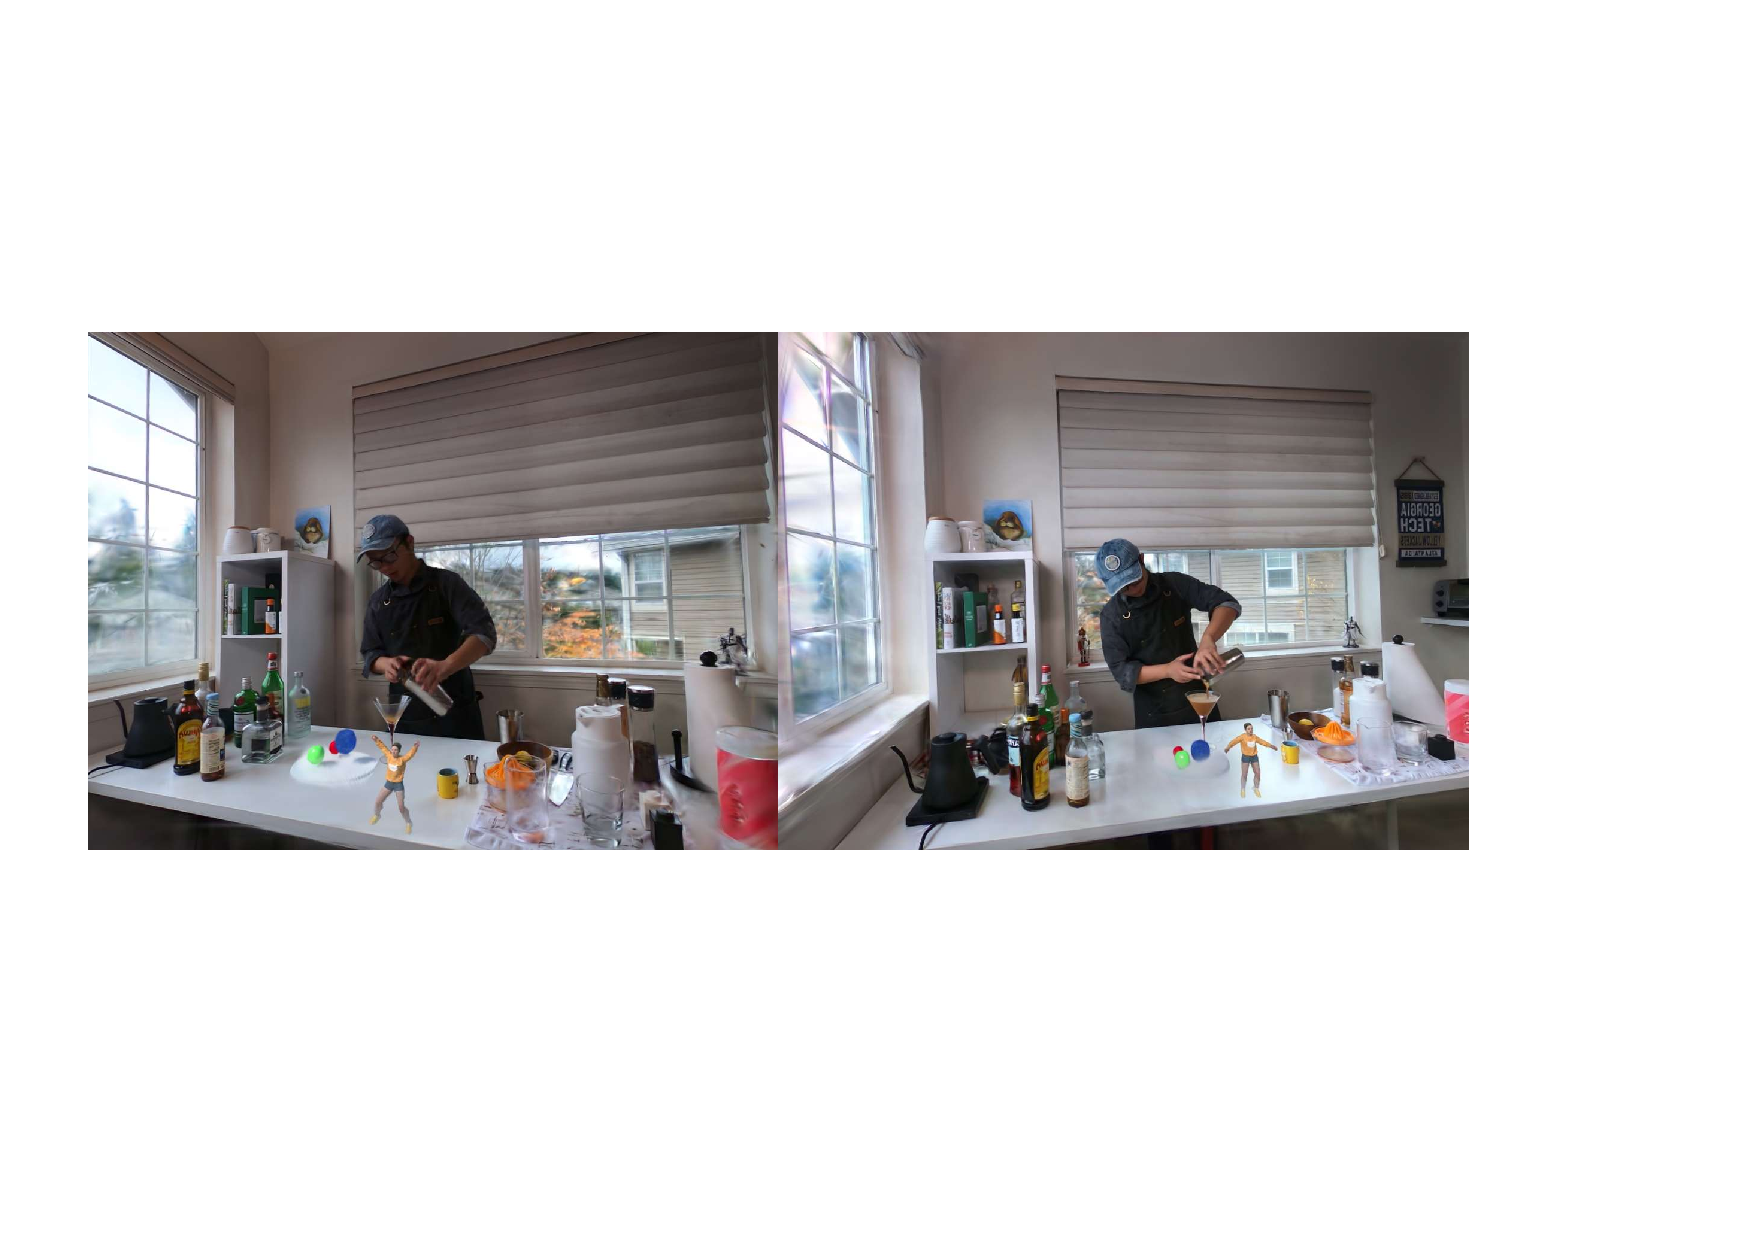
\includegraphics[width=\linewidth]{fig/editing.pdf}
   \caption{Visualization of composition with 4D Gaussians.}
   \label{fig: editing}
   \vspace{-10pt}
\end{figure}
\vspace{-3pt}

\paragraph{Composition with 4D Gaussians.}Similar to dynamic3DGS~\cite{dynamic3dgs}, our proposed methods can also propose editing in 4D Gaussians in Fig.~\ref{fig: editing}. Thanks to the explicit representation of 3D Gaussians, all the trained models can predict deformed 3D Gaussians in the same space following $\mathcal{G}^\prime=\{ \mathcal{G}_1^\prime,\mathcal{G}_2^\prime,...,\mathcal{G}_n^\prime\}$ and differential rendering~\cite{yifan2019differentiablesplatting} can project all the point clouds into viewpoints by $\hat{I} = \mathcal{S}(M,\mathcal{G}^\prime)$.
\begin{figure}
   \centering
   % \vspace{-1pt}
   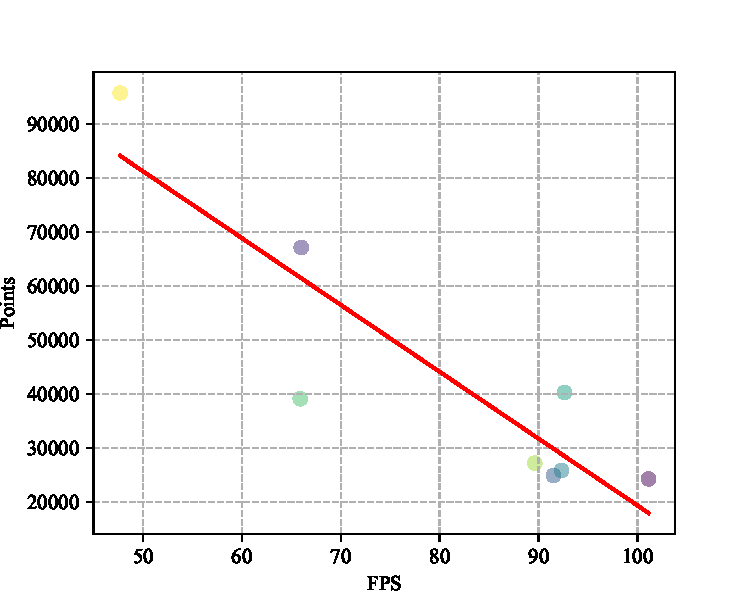
\includegraphics[width=\linewidth]{fig/point_fps.pdf}
   \caption{Visualization of the relationship between rendering speed and numbers of 3D Gaussians in the rendered screens. All the tests are finished in the synthesis dataset.}
    \label{fig:point_fps}
    \vspace{-15pt}
\end{figure}
\vspace{-3pt}
\paragraph{Analysis of Rendering Speed.} As is shown in Fig.~\ref{fig:point_fps}, we also test the relationship between points in the rendered screen and rendering speed at the resolution of 800$\times$800. We found that if the rendered points are lower than 30000, the rendering speed can be up to 90. The config of Gaussian deformation fields are discussed in the appendix. To achieve render-time rendering speed, we should strike a balance among all the rendering resolutions, 4D Gaussians representation including numbers of 3D Gaussians, and the capacity of the Gaussian deformation field network and any other hardware constraints.

% \paragraph{Empty Voxel Mask Grid.}
% For mutli-cams setups, the weight provided by empty voxel mask grid can correct the deformation fields' output, add the mask grid would contribute to PSNR by 0.4 dB. Fig.~\ref{fig: ab_emptyvoxel} shows the difference between training with empoty voxel mask grid or optimizing without it.
% In datasets such as D-NeRF~\cite{pumarola2021dnerf} and DyNeRF~\cite{li2022neural}, there is no prior point cloud information available for initializing 3D Gaussians. Consequently, training the model to learn both 3D Gaussians and deformation fields becomes considerably more challenging compared to static scenes. To address this issue, we adopt the strategy of optimizing 3D Gaussians exclusively, allowing the model to establish a suitable initialization for learning the motion fields. As illustrated in Fig.~\ref{fig: ab_coarse2fine}, through a brief static training stage of just $N=3000$ iterations (lasting no more than 2 minutes), we observe a notable improvement of approximately 1.5 dB in the PSNR of the scene.

% Conversely, eliminating the 8x upsampling resolution negatively impacts the results, demonstrating its critical role in maintaining rendering quality.

% \paragraph{Fast Training.}Conversely, stopping the model's training at iteration 7k can still yield relatively good results, this approach has the potential to train a faster coarse model. The results of fast training are also displayed in Tab.~\ref{table_ab}.

% \paragraph{Image-based Loss.}
% We owe a significant portion of our progress to the splatting algorithm. In every training stage, an image is generated by the model based on the provided training camera pose. This allows us to apply LPIPS-based~\cite{lpips} Loss and SSIM-based~\cite{ssim} Loss during the training process. However, it's essential to acknowledge that this inclusion does slow down the training speed by over 2 times, potentially impeding real-time rendering. It may be because optimizing the motion part is a hard and complex process. Adding image-based loss may trigger worse cases. As a result, during the training stage, we have chosen to decelerate this process to ensure more efficient model training.


% \begin{figure}
%    \centering
%    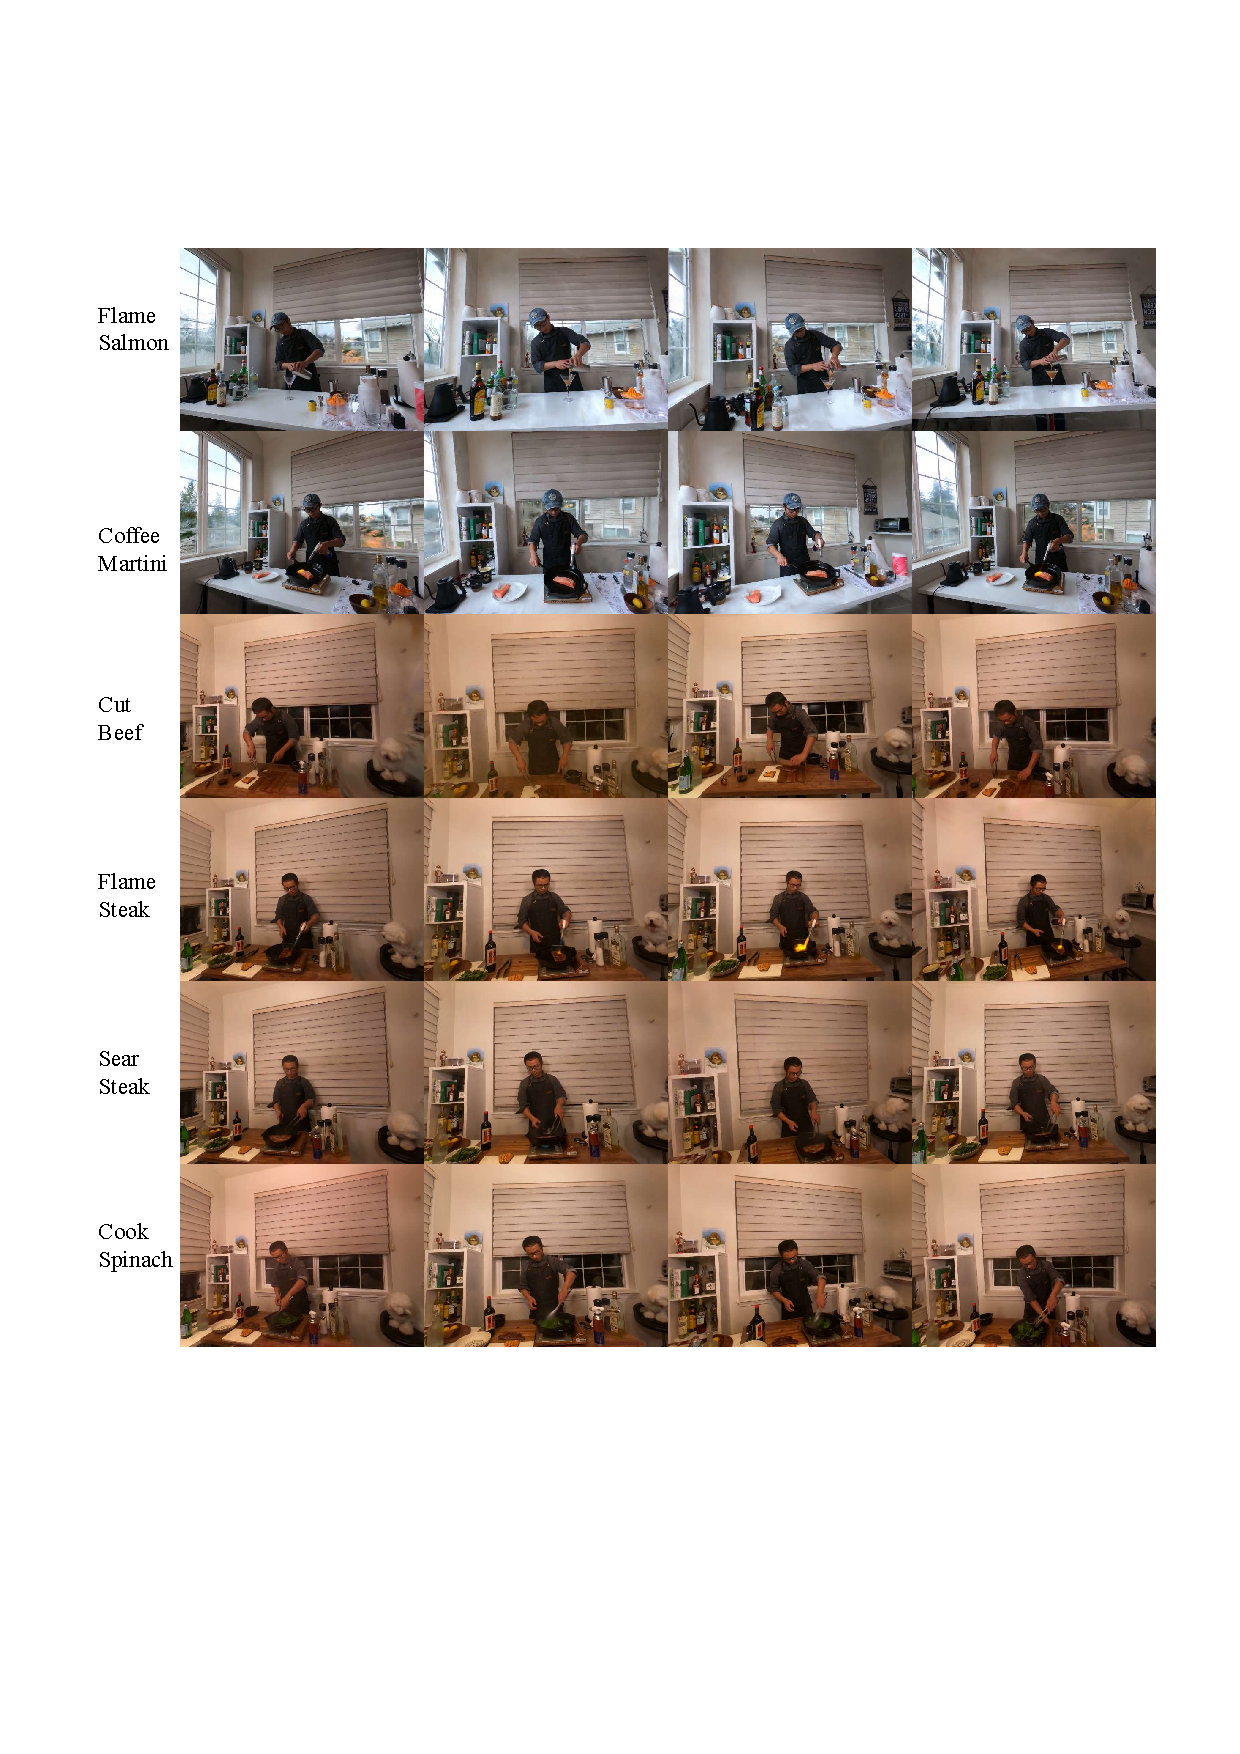
\includegraphics[width=1.0\linewidth]{fig/dynerf_result.pdf}
%    \caption{Visualization of DyNeRF's rendering results through our model, as referenced in \cite{li2022neural}.}
%       \label{fig: dynerf_result}

% \end{figure}
\subsection{Limitations}
\label{Subsec:limitation}
Though 4D-GS can indeed attain rapid convergence and yield real-time rendering outcomes in many scenarios, there are a few key challenges to address. First, large motions, the absence of background points, and the unprecise camera pose cause the struggle of optimizing 4D Gaussians. What is more, it is still challenging to 4D-GS also cannot split the joint motion of static and dynamic Gaussiansparts under the monocular settings without any additional supervision. Finally, a more compact algorithm needs to be designed to handle urban-scale reconstruction due to the heavy querying of Gaussian deformation fields by huge numbers of 3D Gaussians. 

\section{Conclusion}
This paper proposes 4D Gaussian splatting to achieve real-time dynamic scene rendering. An efficient deformation field network is constructed to accurately model Gaussian motions and shape deformations, where adjacent Gaussians are connected via a spatial-temporal structure encoder. Connections between Gaussians lead to more complete deformed geometry, effectively avoiding avulsion. Our 4D Gaussians can not only model dynamic scenes but also have the potential for 4D objective tracking and editing.
% an advanced dynamic scene reconstruction algorithm capable of delivering high-quality results while enabling real-time rendering. While Gaussian representation proves effective for achieving high-quality rendering results in indoor environments, it's important to note that the omission of background point modeling remains an area of interest and warrants further investigation.









